\scanpage{54}
\noindent\begin{minipage}[t]{.47\linewidth}
\figure{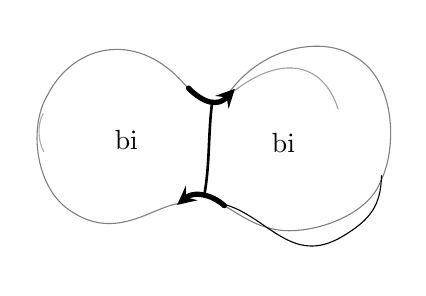
\begin{tikzpicture}[x=.0095cm,y=-.0095cm,line cap=round,line join=round]
  \draw[gray] (278,145) .. controls (213,64) and (125,84) .. (90,153) .. controls (64,195) and (73,279) .. (122,309) .. controls (181,348) and (228,304) .. (265,298);
  \draw[gray!65] (84,178) .. controls (75,194) and (78,218) .. (85,229);
  \draw[gray] (333,149) .. controls (380,86) and (458,76) .. (497,100) .. controls (556,130) and (557,225) .. (535,268) .. controls (517,317) and (438,341) .. (395,333) .. controls (365,328) and (344,311) .. (319,297);
  \draw[gray!75] (339,148) .. controls (402,99) and (458,109) .. (478,172);
  \draw (325,299) .. controls (384,315) and (416,383) .. (484,342) .. controls (521,320) and (535,301) .. (536,261);
  \draw[line width=.95pt] (310,161) .. controls (304,204) and (307,246) .. (299,288);
  \draw[line width=1.9pt,->,>=stealth] (278,144) .. controls (298,164) and (317,169) .. (340,145);
  \draw[line width=1.9pt,->,>=stealth] (326,301) .. controls (308,285) and (285,282) .. (263,300);
  \node at (195,213) {bi}; \node at (405,217) {bi};
\end{tikzpicture}}
\unsure{attachement|Attachement} de deux arêtes \deleted{\unsure{birives|bifidées}}\unsure{bifides} : on trouve \deleted{deux} \inserted{paire d'}arêtes \deleted{opposées} \inserted{$\unsure{a|e},a'$ \uline{\unsure{birives|monorives|bivives}}} qui sont tels que $(a,\omega)\unsure{,}(a',\omega)$ et $(a,\bar{\omega}),(a',\bar{\omega})$ sont des \inserted{\deleted{\unsure{paire|paires}} d'}arcs associés, \deleted{\unsure{mais}} \[\begin{aligned}f&=f'\unsure{+|-}f''-2\\ g&=g'+g''\end{aligned}\ \left|\begin{aligned}&4\ \text{faces}\\ &\text{deviennent }2\end{aligned}\right.\]
\end{minipage}\hfill\begin{minipage}[t]{.50\linewidth}
\figure{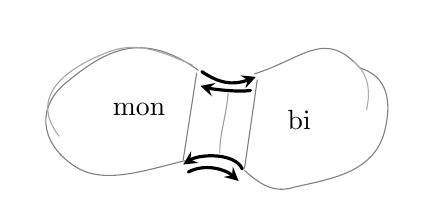
\begin{tikzpicture}[x=.0095cm,y=-.0095cm,line cap=round,line join=round]
  \draw[gray] (1075,177) .. controls (1000,123) and (951,151) .. (902,191) .. controls (857,225) and (864,274) .. (908,304) .. controls (946,331) and (1000,312) .. (1057,298);
  \draw[gray!70] (889,265) .. controls (848,212) and (898,174) .. (957,152) .. controls (995,138) and (1031,154) .. (1067,170);
  \draw[gray] (1150,182) .. controls (1215,162) and (1244,121) .. (1291,174) .. controls (1320,183) and (1337,207) .. (1324,259) .. controls (1309,317) and (1245,323) .. (1201,334) .. controls (1176,341) and (1158,330) .. (1137,311);
  \draw[gray!65] (1282,165) .. controls (1304,182) and (1305,207) .. (1300,230);
  \draw[gray] (1073,181) -- (1055,297) (1154,190) -- (1137,308); \draw[gray!75] (1115,208) .. controls (1113,237) and (1103,264) .. (1104,288);
  \draw[line width=1.15pt,->,>=stealth] (1080,179) .. controls (1102,194) and (1121,198) .. (1152,186);
  \draw[line width=1.15pt,->,>=stealth] (1145,204) .. controls (1129,207) and (1092,202) .. (1078,198);
  \draw[line width=1.15pt,->,>=stealth] (1134,309) .. controls (1124,287) and (1077,289) .. (1055,303);
  \draw[line width=1.15pt,->,>=stealth] (1062,313) .. controls (1085,301) and (1112,310) .. (1129,325);
  \node at (996,230) {mon}; \node at (1210,244) {bi};
\end{tikzpicture}}
Attachement de deux arêtes, l'une \unsure{monorive|monovive}, l'autre birive. On trouve \unsure{paire|pair} d'arêtes $\{a,a'\}$ \unsure{(}\deleted{\unsure{birives}}\inserted{monorives}) incidentes \unsure{:|à} une \unsure{$=$} face \[\begin{aligned}f^{\unsure{\ast|\prime}}&=f'+f''-2\\ g&=g'\unsure{-|+}g''\end{aligned}\ \left|\begin{aligned}&\text{\unsure{trois|deux} faces}\\ &\text{deviennent }1\end{aligned}\right.\]
\end{minipage}

\figure{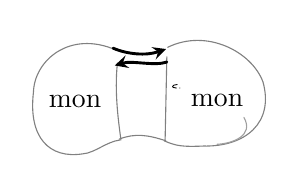
\begin{tikzpicture}[x=.011cm,y=-.011cm,line cap=round,line join=round]
  \draw[gray] (775,937) .. controls (722,914) and (681,949) .. (680,986) .. controls (674,1038) and (698,1063) .. (737,1057) .. controls (751,1056) and (764,1043) .. (780,1041);
  \draw[gray] (835,934) .. controls (880,912) and (932,939) .. (945,974) .. controls (958,1021) and (925,1049) .. (876,1048) .. controls (852,1049) and (845,1048) .. (831,1042);
  \draw[gray!75] (923,1015) .. controls (935,1036) and (910,1045) .. (892,1046);
  \draw[gray] (777,952) .. controls (773,987) and (779,1025) .. (781,1041) (834,945) -- (832,1042) (779,1040) .. controls (797,1033) and (812,1035) .. (833,1042);
  \draw[line width=1.05pt,->,>=stealth] (772,935) .. controls (788,942) and (810,944) .. (833,936);
  \draw[line width=1.05pt,->,>=stealth] (834,951) .. controls (820,956) and (794,949) .. (774,955);
  \node at (728,997) {mon}; \node at (892,995) {mon}; \draw[line width=.32pt] (846,977) .. controls (840,977) and (838,981) .. (845,981); \fill (849,981) circle (.6);
\end{tikzpicture}}
Attachement de deux arêtes \deleted{\unsure{bifides|bifidées}}\unsure{monorives} on trouve \deleted{deux} paire d'arêtes monorives, incidentes à des faces distinctes

\noindent\begin{minipage}[c]{.46\linewidth}
\[\begin{aligned}f&=f'+f''\\ \underline{g}&=g'+g''-1\end{aligned}\]
\end{minipage}\hfill\begin{minipage}[c]{.51\linewidth}
\figure{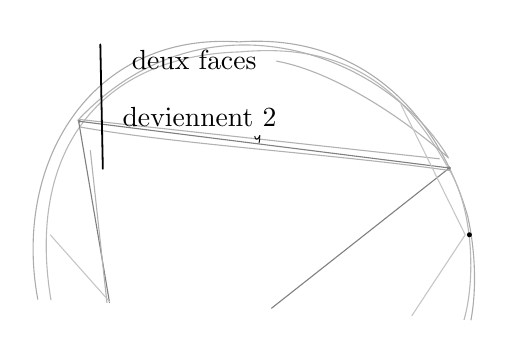
\begin{tikzpicture}[x=.0106cm,y=-.0106cm,line cap=round,line join=round]
  \clip (946,1308) -- (1489,1308) -- (1489,1659) -- (945,1633) -- cycle;
  \draw[gray!65] (958,1638) .. controls (925,1473) and (1019,1313) .. (1198,1325) .. controls (1335,1315) and (1433,1400) .. (1472,1534) .. controls (1483,1584) and (1482,1633) .. (1474,1667);
  \draw[gray!55] (975,1646) .. controls (940,1465) and (1024,1342) .. (1199,1337) .. controls (1321,1326) and (1392,1374) .. (1448,1475) .. controls (1478,1521) and (1483,1611) .. (1466,1663);
  \draw[gray!60] (1005,1419) .. controls (1156,1258) and (1373,1337) .. (1449,1464) .. controls (1396,1417) and (1313,1361) .. (1243,1348);
  \draw[gray] (1006,1420) -- (1450,1476) -- (1237,1644) (1006,1420) -- (1043,1637);
  \draw[gray!60] (1008,1427) .. controls (1126,1448) and (1310,1459) .. (1450,1479) (1008,1418) -- (1438,1465) (1020,1455) -- (1040,1638);
  \draw[gray!45] (972,1556) -- (1043,1636) (1392,1400) -- (1469,1556) -- (1405,1653);
  \fill[gray] (1007,1420) circle (2) (1450,1476) circle (2); \fill (1474,1556) circle (3);
  \draw[line width=.65pt] (1032,1328) -- (1035,1477);
  \node[anchor=west] at (1058,1346) {deux faces};
  \node[anchor=west] at (1047,1415) {deviennent $2$};
  \draw[line width=.33pt] (1217,1438) .. controls (1217,1441) and (1220,1445) .. (1223,1437) .. controls (1224,1440) and (1222,1444) .. (1222,1446);
\end{tikzpicture}}
\end{minipage}
% archive sheet number: 53

